\section{Dario e Xerxes}

\begin{frame}[fragile]{Problema}

A brincadeira da Pedra, Papel e Tesoura, muita gente conhece. Mas dá para fazer uma mais legal com
cinco opções e não só três! Dois jogadores, \texttt{dario} e \texttt{xerxes}, jogam uma partida
com $N$ rodadas. Em cada rodada os jogadores escolhem uma ``mão'' entre cinco opções, que vamos
representar aqui com os números 0, 1, 2, 3 e 4. A figura define exatamente quem ganha a rodada. Por
exemplo, se \texttt{dario} escolheu 0 e \texttt{xerxes} escolheu 3, então \texttt{xerxes} ganha a
rodada, pois existe uma seta na figura indo de 3 para 0.

\end{frame}

\begin{frame}[fragile]{Problema}

    \begin{figure}[!ht]
        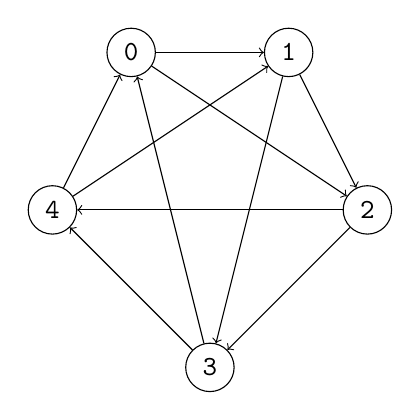
\begin{tikzpicture}
            \node[draw,circle] (A) at (2, 4) { \texttt{0} };
            \node[draw,circle] (B) at (4, 4) { \texttt{1} };
            \node[draw,circle] (C) at (5, 2) { \texttt{2} };
            \node[draw,circle] (D) at (3, 0) { \texttt{3} };
            \node[draw,circle] (E) at (1, 2) { \texttt{4} };

            \draw[->] (A) edge (B);
            \draw[->] (A) edge (C);
            \draw[->] (B) edge (C);
            \draw[->] (B) edge (D);
            \draw[->] (C) edge (D);
            \draw[->] (C) edge (E);
            \draw[->] (D) edge (E);
            \draw[->] (D) edge (A);
            \draw[->] (E) edge (A);
            \draw[->] (E) edge (B);

        \end{tikzpicture}
    \end{figure}

\end{frame}

\begin{frame}[fragile]{Problema}

Depois de $N$ rodadas, o vencedor da partida é o jogador que ganhou mais rodadas. O número $N$
será sempre ímpar, para não haver empate na partida. Vamos também considerar que os jogadores nunca
escolhem a mesma mão numa rodada, para não haver empate na rodada. Você deve escrever um programa
que determine quem venceu a partida, se foi \texttt{dario} ou \texttt{xerxes}.

\end{frame}

\begin{frame}[fragile]{Entrada e saída}

\textbf{Entrada}

A primeira linha da entrada contém um inteiro $N$, o número de rodadas na partida. Cada uma das
$N$ linhas seguintes contém dois inteiros $D$ e $X$, representando a mão que os jogadores dario e
xerxes, respectivamente, jogaram em uma rodada.

\end{frame}

\begin{frame}[fragile]{Entrada e saída}

\textbf{Saída}

Seu programa deve imprimir uma linha contendo o nome do jogador que venceu a partida:
\texttt{dario} ou \texttt{xerxes}. Todas as letras devem ser minúsculas, sem nenhum acento!

\vspace{0.1in}

\textbf{Restrições}

\begin{itemize}
    \item $1\leq N\leq 999$, $N$ é impar
    \item $0\leq D, X\leq 4$ e $D\neq X$
\end{itemize}

\end{frame}

\begin{frame}[fragile]{Exemplo de entradas e saídas}

\begin{minipage}[t]{0.45\textwidth}
\textbf{Entrada}
\begin{verbatim}
3
1 3
4 2
0 2


1
3 1
\end{verbatim}
\end{minipage}
\begin{minipage}[t]{0.5\textwidth}
\textbf{Saída}
\begin{verbatim}
dario





xerxes
\end{verbatim}
\end{minipage}
\end{frame}

\begin{frame}[fragile]{Solução}

    \begin{itemize}
        \item Como o problema excluí a possibilidade de ambos escolherem o mesmo número,
            há 20 jogadas possíveis

        \item Testar cada uma destas 20 possibilidades, acumulando as vitórias de cada um
            produz uma solução correta, porém de codificação trabalhosa e propensa a erros:

        \vspace{0.1in}
        \inputsyntax{cpp}{codes/dario_bf.cpp}

    \end{itemize}

\end{frame}

\begin{frame}[fragile]{Solução}

    \begin{itemize}
        \item Uma maneira de se eliminar a metade destas condicionais é observar que, caso Dario
            não vença, Xerxes será o vencedor

        \item Além disso, todas as 10 condições podem ser combinadas em uma única condição, por
            meio do operador lógico \texttt{OU}

        \vspace{0.1in}
        \inputsyntax{cpp}{codes/dario_ifs.cpp}

    \end{itemize}

\end{frame}

\begin{frame}[fragile]{Solução}

    \begin{itemize}
        \item Uma vez que não há possibilidade de empate, não é preciso contabilizar as vitórias
            de Xerxes, pois \code{cpp}{xerxes = N - dario}

        \item Além disso, Dario será o vencedor da disputa apenas se vencer mais da metade de todas
            as rodadas, isto é, se \code{cpp}{dario > N/2}

        \item A observação cuidadosa do texto e das dez condicionais apresentadas mostra que um
            número \code{cpp}{x} vence seus dois sucessores, se considerados apenas seus restos
            da divisão por 5

        \item Assim, a condição de vitória de Dario se reduz a

        \vspace{0.1in}
        \inputsyntax{cpp}{codes/dario_mod.cpp}

    \end{itemize}

\end{frame}

\begin{frame}[fragile]{Solução $O(N)$}
    \inputsnippet{cpp}{1}{21}{codes/dario.cpp}
\end{frame}
